\documentclass[a4paper,10pt]{article}

%%%%%%%%%%%%%%%%%%%%%%%%%%%%%%%%%%%%%%%%%%%%%%%%%%%%%%%%%%%%%%%%%%%%%%%%%%%%%%%%
%%% Package selection
%%%%%%%%%%%%%%%%%%%%%%%%%%%%%%%%%%%%%%%%%%%%%%%%%%%%%%%%%%%%%%%%%%%%%%%%%%%%%%%%

% Language and encoding packages
\usepackage[utf8]{inputenc} % Accept utf8 encoded files.
\usepackage[T1]{fontenc}    % Text encoding.
\usepackage[english]{babel} % Mmultilingual for characters characters.

%%% Figure realted packages
\usepackage{caption}    % Caption customization.
\usepackage{subcaption} % More caption tools.
\usepackage{float}      % Improved options for floats/figs.
\usepackage{minted}     % For syntax highlighting code.
\usepackage{tikz}       % For creating diagrams.

%%% Misc Packages
\usepackage[lang=en,grid]{kufront} % KU Front page package.
\usepackage{todonotes}             % For enabling the \todo command.
\usepackage{mdwlist}               % For itemize* and enumerate* environments.
\usepackage{pdflscape}             % Allows landscape pages.

%%%%%%%%%%%%%%%%%%%%%%%%%%%%%%%%%%%%%%%%%%%%%%%%%%%%%%%%%%%%%%%%%%%%%%%%%%%%%%%%
%%% Type setting and own commands
%%%%%%%%%%%%%%%%%%%%%%%%%%%%%%%%%%%%%%%%%%%%%%%%%%%%%%%%%%%%%%%%%%%%%%%%%%%%%%%%

% What parts of the tikz package do we want to load?
\usetikzlibrary{arrows,shapes,positioning,shadows,trees}

%Styleset for organization diagram.
\tikzset{
  basic/.style  = {draw, text width=2cm, drop shadow, font=\sffamily, rectangle},
  board/.style   = {basic, rounded corners=2pt, thin, align=center,
                   fill=white!30},
  officer/.style = {basic, rounded corners=6pt, thin,align=center, fill=white!60,
                   text width=8em},
  department/.style = {basic, rounded corners=6pt, thin,align=center, fill=white!60,
                   text width=8em},
  employee/.style = {basic, thin, align=left, fill=pink!60, text width=6.5em}
}

% Use sans-serif font for KU logo.
\renewcommand{\kufrontfont}{\sffamily}

% Redefine \theFancyVerbLine to enable line numbers in minted.
\renewcommand{\theFancyVerbLine}{\sffamily
\textcolor[rgb]{0.5,0.5,1.0}{\scriptsize
\oldstylenums{\arabic{FancyVerbLine}}}}

% Line used for the abstract.
% Usage: \HRule
\newcommand{\HRule}{\rule{\linewidth}{0.5mm}}

% Displays a centered image with caption and label.
% usage: \graphicc{width}{file}{caption}{label}
\newcommand{\graphicc}[4]{\begin{figure}[H] \centering
            \includegraphics[width={#1\textwidth}, keepaspectratio=true]{{#2}}
            \caption{{#3}} \label{#4} \end{figure}}

% Load some code from a file and display it in a pretty figure.
% usage: \codefig{language}{file}{firstline}{lastline}{caption}{label}
\newcommand{\codefig}[6]
{
\begin{figure}[H]
    \inputminted[firstnumber=#3,firstline=#3,lastline=#4,
                 linenos=true]{#1}{#2}
    \caption{#5 (#2)}
    \label{code:#6}
\end{figure}
}

%%%%%%%%%%%%%%%%%%%%%%%%%%%%%%%%%%%%%%%%%%%%%%%%%%%%%%%%%%%%%%%%%%%%%%%%%%%%%%%%
%%% Meta information for the KU front page.
%%%%%%%%%%%%%%%%%%%%%%%%%%%%%%%%%%%%%%%%%%%%%%%%%%%%%%%%%%%%%%%%%%%%%%%%%%%%%%%%

\title{User Behavior Analysis Using Decision Trees}
\author{\Large Martin Nicklas Jørgensen \quad {\ttfamily\large tzk173@alumni.ku.dk}}
\date{\today}
\project{\mdseries\LARGE Company Project \# 2015-1428}
\supervisor{Supervisor: Mikkel Rønne Jakobsen \quad {\ttfamily\large mikkelrj@di.ku.dk}}

%%%%%%%%%%%%%%%%%%%%%%%%%%%%%%%%%%%%%%%%%%%%%%%%%%%%%%%%%%%%%%%%%%%%%%%%%%%%%%%%
% Start the actual document.
%%%%%%%%%%%%%%%%%%%%%%%%%%%%%%%%%%%%%%%%%%%%%%%%%%%%%%%%%%%%%%%%%%%%%%%%%%%%%%%%

\begin{document}

% Create the front page.
\begin{titlepage}
\maketitle
\end{titlepage}

% Insert an abstract.
\hspace{1cm}\\[5cm]
{\huge Abstract}
\\\HRule\\
\todo[inline]{Write something sensible.}
Lorem ipsum dolor sit amet, consectetur adipiscing elit. Donec a diam lectus.
Sed sit amet ipsum mauris. Maecenas congue ligula ac quam viverra nec
consectetur ante hendrerit. Donec et mollis dolor. Praesent et diam eget libero
egestas mattis sit amet vitae augue. Nam tincidunt congue enim, ut porta lorem
lacinia consectetur. Donec ut libero sed arcu vehicula ultricies a non tortor.
Lorem ipsum dolor sit amet, consectetur adipiscing elit. Aenean ut gravida
lorem. Ut turpis felis, pulvinar a semper sed, adipiscing id dolor. Pellentesque
auctor nisi id magna consequat sagittis. Curabitur dapibus enim sit amet elit
pharetra tincidunt feugiat nisl imperdiet. Ut convallis libero in urna ultrices
accumsan. Donec sed odio eros. Donec viverra mi quis quam pulvinar at malesuada
arcu rhoncus. Cum sociis natoque penatibus et magnis dis parturient montes,
nascetur ridiculus mus. In rutrum accumsan ultricies. Mauris vitae nisi at sem
facilisis semper ac in est.

\newpage

\tableofcontents

% actual report sections.
\section{Introduction}
                % Inroduction to the project.
\section{Simplesite ApS}


%%%%%%%%%%%%%%%%%%%%%%%%%%%%%%%%%%%%%%%%%%%%%%%%%%%%%%%%%%%%%%%%%%%%%%%%%%%%%%%%
\subsection{Product}

Simplesite produce and manage an inhouse website Content Management System (CMS)
and operate a hosting location where this CMS runs. Customers can register for a
free account allowing them to host a website that is edited through the CMS. The
free accounts are under restrictins on number fo pages, images and videos that
can be added to the site. Customers can then change to a paid subscription which
allows them to have more pages, images and videos on their website.

Simplesite also offer additional services to their customers that can be bought
for an extra fee if you are already a paying customer, this includes the ability
to have a domain attached to your website, a webshop as well as more additional
pages, images and videos.

The product is hosted partially on Simplesites own hardware in an offsite
location, and using a number of cloud services to provide faster response times
for certain data types.


%%%%%%%%%%%%%%%%%%%%%%%%%%%%%%%%%%%%%%%%%%%%%%%%%%%%%%%%%%%%%%%%%%%%%%%%%%%%%%%%
\subsection{Departments}

\begin{itemize*}
    \item \textbf{Administration} - Situated at the ground floor of the
          Copenhagen office, this department contains the HR functions as well
          as finance.

    \item \textbf{Sales} - Also on the ground floor of the Copenhagen office,
          sales consists of full time employeess and student helpers. The
          primary task is to sell the product, currently through localized ad
          management.

    \item \textbf{P \& C}\footnote{Product and Communication.} - The department
          sits on the upper floor of the Copenhagen office and is responsible
          for planning new features in cooperation with the developers as well
          as manage content on Simplesites own websites. P \& C also manages
          communication such as newsletters and localized ad texts.

    \item \textbf{In-House Development} - Sitting next to P \& C on the upper
          floor the developers are responsible for implementing new features as
          well as maintenence, analytics and bug fixing of the product.

    \item \textbf{Operations} - Daily operations are handled primarily by the
          company CTO, Thomas, as well as 2 part time students, operations sits
          on the upper floor in Copenhagen next to the developers.

    \item \textbf{Support} - Since the product is offered in several languages,
          a supporter is hired per language in a part time basis. All supporters
          work from home but get together once a month for a status meeting and
          to make sure new knowledge is shared and that relevant information can
          be given from the regular departments.

    \item \textbf{Remote Dev 1} - A small number of developers are hired in
          Bulgaria and have their own office in the Sofia, they are offered
          machines in the Copenhagen office they can VPN into and use for work.
          This allows the operations department to work from Copenhagen and
          still service the remote developers.

    \item \textbf{Remote Dev 2} - A number of developers are also hired from
          Serbia, like the remote developers in Bulgaria, they also VPN into the
          Copenhagen office and work on machines maintained by the regular
          operations employees.

    \item \textbf{Miscellaneous} - Simplesite also occasionally employs external
          specialists or consultants. Depending on the need, they will either
          work in the Copenhagen office or from some remote location using VPN.
\end{itemize*}


%%%%%%%%%%%%%%%%%%%%%%%%%%%%%%%%%%%%%%%%%%%%%%%%%%%%%%%%%%%%%%%%%%%%%%%%%%%%%%%%
\subsection{Company Structure}


\begin{landscape}
\todo[inline]{Double check names and titles.}
\begin{figure}[H]
\centering
\hspace*{-2cm}
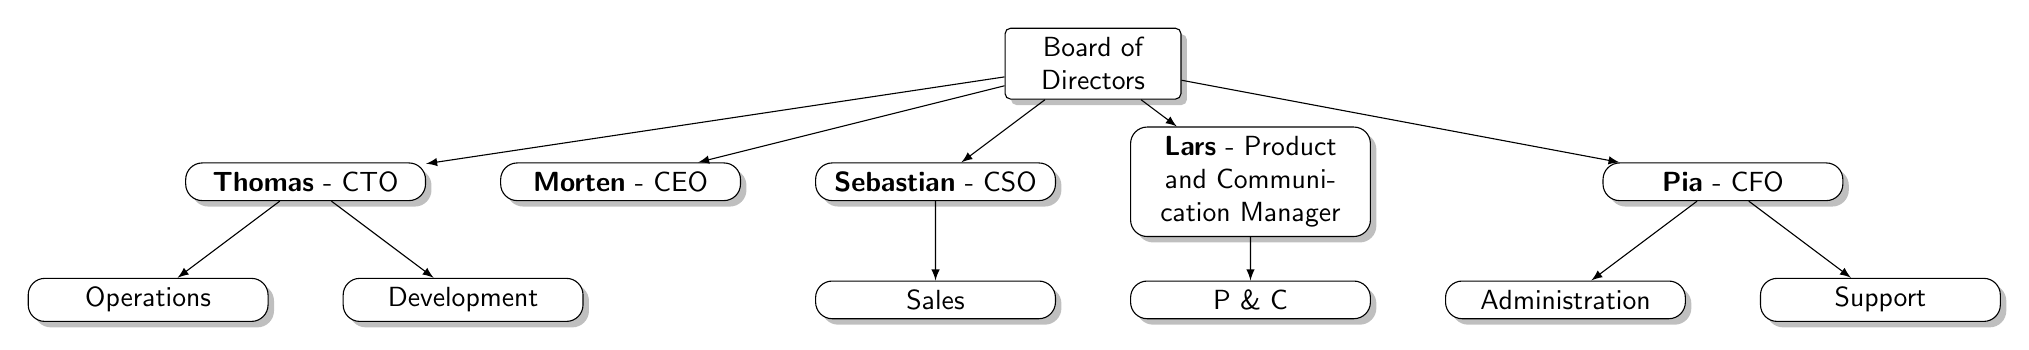
\begin{tikzpicture}[
  level 1/.style={sibling distance=40mm},
  edge from parent/.style={->,draw},
  >=latex]

% root of the the initial tree, level 1
\node[board] {Board of Directors}
% The first level, as children of the initial tree
  child {node[officer] (c2) {\textbf{Thomas} - CTO}
    child{node[department] (c21) {Operations}}
    child{node[department] (c22) {Development}}
  }
  child {node[officer] (c1) {\textbf{Morten} - CEO}}
  child {node[officer] (c3) {\textbf{Sebastian} - CSO}
    child{node[department] (c31) {Sales}}
  }
  child {node[officer] (c5) {\textbf{Lars} - Product and Communication Manager}
    child{node[department] (c51) {P \& C}}
  }
  child[missing]
  child {node[officer,xshift=-2cm] (c4) {\textbf{Pia} - CFO}
    child{node[department] (c41) {Administration}}
    child{node[department] (c42) {Support}}
  };

\end{tikzpicture}

\caption{Organizational diagram for Simplesite ApS}
\label{fig:orgdiagram}
\end{figure}
\end{landscape}     % Description of the company structure and workflow.
\section{Problem Description}         % Description of the problem.
\section{Problem Analysis}

In order to work with the the problem described in Section \ref{sec:probdesc} I
used a workflow called called the \textit{Cross Industry Standard Process for
Data Mining}, shortened to CRISP-DM (as described in \cite[p.
26]{provost2013data}, originally from \cite{shearer2000crisp}). An overview of
the process can be seen in Figure \ref{fig:crisp}. The following subsections
will go over each phase in the process, explaining what the purpose of the phase
is and cover my work during that phase of the project.

\graphicc{0.8}{img/wiki_crisp}{Diagram of the CRISP-DM method. Source:
  \cite{wiki2016crisp}.}{fig:crisp}

Simplesite have performed most of the \textit{business understanding} step so
the work I performed is placed in \textit{data understanding}, \textit{data
preparation}, \textit{modelling} and \textit{evaluation}. Due to the short
duration of the project, there have not been any time spent with the
\textit{deployment} phase.


%%%%%%%%%%%%%%%%%%%%%%%%%%%%%%%%%%%%%%%
\subsection{Business Understanding}

The business understanding phase is the entry point for most data science
projects, it covers the process of taking a business project, and converting it
to a data science project. My work in the phase have been very limited, since
Simplesite had a very clear idea of what they would like to investigate first.
The initial business problem for this project can be described as ``\textit{We
have a large number of free users, but a lot of them do not stay with the
product. Can we find out why?}''. From this business problem it makes sense to
ask ``\textit{Can we find a difference between the customers that stay and those
who don't?}'', more specifically is there a difference in the way the customer
behave when using the site? And that question is what this project is being
performed from.


%%%%%%%%%%%%%%%%%%%%%%%%%%%%%%%%%%%%%%%%%%%%%%%%%%%%%%%%%%%%%%%%%%%%%%%%%%%%%%%%
%%%%%%%%%%%%%%%%%%%%%%%%%%%%%%%%%%%%%%%%%%%%%%%%%%%%%%%%%%%%%%%%%%%%%%%%%%%%%%%%
\subsection{Data Understanding}


The data understanding phase of data science is the second phase. During this
phase you look into what data is available and collect whatever information
might be relevant for the data science problem. During this phase you will also
identify data quality problems and gain familiarity with the data in order to
help form a better hypothesis. It is worth noting that weaknesses in the dataset
are not removed until the next phase, data preparation, so in order to make the
report more readable, any arguments for removal or change will be listed in
Section \ref{sec:datasetpruning} instead of here.

The basis for the analysis is 2 datasets created by Simplesite:
\texttt{EngagementData} \& \texttt{CustomerJourney}. Table
\ref{tab:engdatalayout} and Table \ref{tab:cjdatalayout} names the features of
each dataset and what they represent. Both datasets contain users created
between September 1st 2015 and September 30 2015. The data is recorded for all
users after this point as well, but the larger dataset also increases memory
consumption, and makes it unwieldy. The training datasets both contain $463716$
observations, each corresponding to a user created in this timespan.

Another copy of each dataset was created from the database pulling data from
users created between October 1st 2015 and October 30 2015. These datasets
contains $495390$ observations and will be used as test data.

\begin{table}[H]
    \centering
    \begin{tabularx}{\textwidth}{l|X}
        \textbf{Attribute Name} & \textbf{Attribute Data}                                                                                                     \\ \hline
        \textit{islogins1}                       & Bool, true if: one or more logins for the user.                                                            \\
        \textit{islogins2}                       & Bool, true if: two or more logins for the user.                                                            \\
        \textit{islogins3}                       & Bool, true if: three or more logins for the user.                                                          \\
        \textit{islogins4}                       & Bool, true if: four or more logins for the user.                                                           \\
        \textit{isedit30m}                       & Bool, true if: User edited site within 30 minutes of creation.                                             \\
        \textit{isedit24h}                       & Bool, true if: User edited site within 24 hours of creation (excluding the first 30 minutes).              \\
        \textit{isaddpage30m}                    & Bool, true if: User added a new page within 30 minutes of creation.                                        \\
        \textit{isaddpage24h}                    & Bool, true if: User added a new page within 24 hours of creation (excluding the first 30 minutes).         \\
        \textit{isimgupload30m}                  & Bool, true if: User uploaded their own image within 30 minutes of creation.                                \\
        \textit{isimgupload24h}                  & Bool, true if: User uploaded their own image within 24 hours of creation (excluding the first 30 minutes). \\
        \textit{iseditdesign30m}                 & Bool, true if: User edited site within 30 minutes of creation.                                             \\
        \textit{iseditdesign24h}                 & Bool, true if: User edited site within 24 hours of creation (excluding the first 30 minutes).              \\
        \textit{customerid}                      & Integer value with the customers unique ID.                                                                \\
        \textit{marketname}                      & String with the market the user came from (US, TR, DK etc.)                                                \\
        \textit{siteverkey}                      & String with what version of the site the user is created in (US, TR, DK etc.)                              \\
        \textit{ispayer}                         & Bool, true if: The customer have a paid subscription.                                                      \\
        \textit{culturekey}                      & String with language information for the site (en-US, fr-FR etc.)
    \end{tabularx}
    \caption{Features found in the \texttt{EngagementData} dataset.}
    \label{tab:engdatalayout}
\end{table}


\begin{table}[H]
    \centering
    \begin{tabularx}{\textwidth}{l|X}
        \textbf{Attribute Name} & \textbf{Attribute Data}                                                                      \\ \hline
        \textit{customerid}     & Integer value with the customers unique ID.                                                  \\
        \textit{logins14}       & Integer, number of times the customer logged in the first 14 days (week 1-2 after creation). \\
        \textit{logisnw2w4}     & Integer, number of times the customer logged in in week 3-4 after creation.                  \\
        \textit{edits14}        & Integer, number of times the customer edited a page within the first 14 days.                \\
        \textit{iscjtrial}      & Bool, true if: Always true, everyone starts as a trial.                                      \\
        \textit{iscjonboarded}  & Bool, true if: edits14 $\geq 1$.                                                             \\
        \textit{iscjactivated}  & Bool, true if: edits14 $\geq 3$.                                                             \\
        \textit{iscjengaged}    & Bool, true if: edits14 $\geq 6$ and logins14 $\geq 2$.                                       \\
        \textit{iscjinvested}   & Bool, true if: edits14 $\geq 15$ and logins14 $\geq 6$.                                      \\
        \textit{iscjretained}   & Bool, true if: logisnw2w4 $\geq 1$.                                                          \\
        \textit{isimgupload1d}  & Bool, true if: Customer uploaded an image within the first 24 hours of being created.        \\
        \textit{iseditdesign1d} & Bool, true if: Customer edited the design within the first 24 hours of being created.        \\
        \textit{isaddpage1d}    & Bool, true if: Customer added a new page within the first 24 hours of being created.         \\
        \textit{isedit1d}       & Bool, true if: Customer edited a page within the first 24 hours of being created.           
    \end{tabularx}
    \caption{Features found in the \texttt{CustomerJourney} dataset.}
    \label{tab:cjdatalayout}
\end{table}
%%%%%%%%%%%%%%%%%%%%%%%%%%%%%%%%%%%%%%%%%%%%%%%%%%%%%%%%%%%%%%%%%%%%%%%%%%%%%%%%
\subsection{Data Preparation}
\label{sec:datasetpruning}

The data preparation phase is where all the data weaknesses we found in the
previous section is removed and all the raw data is collected into the final
dataset. At the end of this phase the dataset should contain all the data the
models will need and be ready to be ``fed'' to the model for training and
validation.

The initial goal is to find customers who are retained (\textit{iscjretained} =
\texttt{True}), and to see if there is some pattern that Simplesite can use to
try to guide other customers down, in order to increase the number of retained
customers. With this in mind there is some attributes of the datasets that will
not be helpful, either because they cannot be controlled/changed, or because
they do not make sense. The following is a list of attributes removed from the
\texttt{EngeagementData} dataset during work, along with the reason for the
removal.

\begin{itemize*}
    \item \textit{islogins1} : Removed because the knowledge about number of
          logins is contained in the \textit{logins14} feature from the
          \textit{CustomerJourney} dataset.

    \item \textit{islogins2} : Same as \textit{islogins1}.

    \item \textit{islogins3} : Same as \textit{islogins1}.

    \item \textit{islogins4} : Same as \textit{islogins1}.

    \item \textit{marketname} : Removed since we are unable to get a customer from
          a different market, we are insterested in variable we can change for
          each customer.

    \item \textit{siteverkey} : Same as \textit{marketname}.

    \item \textit{ispayer} : Removed because it is an alternative target variable,
          it does not say anything about how the user behaves, other than they are
          indeed a good customer.

    \item \textit{culturekey} : Same as \textit{marketname}.
\end{itemize*}

\noindent The following is a list of attributes removed from the
\texttt{CustomerJourney} dataset during work, along with the reason for the
removal.

\begin{itemize*}
    %\item \textit{logins14} : Removed because initial tests showed high bias. For
    %      a ctree\footnote{Conditional Inference Tree.} of depth 4, the three top
    %      levels was occupied with choices regarding logins14.

    \item \textit{logisnw2w4} : Removed since this attribute is in the definition
          of our target variable \textit{iscjretained}.

    \item \textit{iscjtrial} : Removed since it is always true.

    \item \textit{iscjonboarded} : Removed since it serves as an alternative
          target variable. It is set by Simplesite and does not say anything
          about the user behaviour that is not already present in other
          attributes.

    \item \textit{iscjengaged} : Same as \textit{iscjonboarded}.

    \item \textit{iscjinvested} : Same as \textit{iscjonboarded}.
\end{itemize*}

In both datasets the \textit{customerid} attribute is kept and used to join them
into one training dataset, after this join operation the \textit{customerid}
attribute is removed.

The files \textit{src/dataset\_training.tsv} and \textit{src/dataset\_test.tsv}
contains the data from these final versions of the datasets.

%%%%%%%%%%%%%%%%%%%%%%%%%%%%%%%%%%%%%%%%%%%%%%%%%%%%%%%%%%%%%%%%%%%%%%%%%%%%%%%%
\subsection{Modelling}

During the modelling phase the models are applied to the dataset constructed in
the data preparation phase, and parameters are adjusted to give the best results
possible. Some models might require that the data is in a specific form, so it
might be necessary to step back to the data preparation phase.

\subsubsection{Tree Type}

While researching R, two distinct type of decision trees came up; an
implementation of regular decision trees that closely follow the method
described in \cite{breiman1984classification}, as well as conditional inference
trees\cite{hothorn2006unbiased}, which I will shorten to \textit{ctree} in this
report.

Both models produce binary trees that can be used to solve classification
problems. Each node in the tree represents a variable and each edge out of the
node contains a ``case'' that tells something about the variable (is it
true/false, $\geq 5$, and so forth). Each leaf of the tree is representing a
class, and there can be several leafs with the same class, they just represent
different characteristics of the same class.

The main difference between a regular decision tree and a ctree is how it is
created. A regular decision tree will choose to split using information measures
such as seen in Quinlan et. al.\cite[p. 89]{quinlan1986induction}, whereas the
ctree framework will split based on the relationship between the target feature
and the covariates based on conditional distribution. Given a fresh dataset, a
regular decision tree will make the first split on the attribute where the
resulting split gives the two largest possible subsets on each edge. A
conditional inferance tree on the other hand will split on the
covariate/attribute with the strongest relation to the target variable.


%%%%%%%%%%%%%%%%%%%%%%%%%%%%%%%%%%%%%%%%
\subsubsection{Model Type Precision}
\label{sec:treetypeprecision}

In order to select which tree type to use I performed an experiment that used
5-fold cross validation\cite[p. 32]{bishop2006pattern} to test the accuracy of
the models for different depths. The dataset used for this experiment was the
combination of the \textit{EngagementData} and \textit{CustomerJourney}
datasets, as described in Section \ref{sec:datasetpruning} (excluding the
customerid column.) The code for this test can be seen in Appendix
\ref{app:treecompare} Figure \ref{app:code:treecompare}.

\begin{table}[H]
    \centering
    \begin{tabular}{l|l|l}
        \textbf{Max Depth} & \textbf{\texttt{rpart} Accuracy} & \textbf{\texttt{ctree} Accuracy} \\ \hline
        \textit{4}         & $94.2799$ \%                     & $94.27990$ \%                    \\
        \textit{8}         & $94.2799$ \%                     & $94.31958$ \%                    \\
        \textit{12}        & $94.2799$ \%                     & $94.36638$ \%
    \end{tabular}
    \caption{The mean accuracy for the different 5-fold cross validation runs.}
    \label{tab:treecompare}
\end{table}

The results shown in Table \ref{tab:treecompare} indicates that for our
particular dataset, the accuracy difference for the two models is very
insignificant. They both predict correctly in around $94,3\%$ of the cases with
a difference of less that $0,1\%$ between the best and worst performer.

An interesting observation from the data above is that the \texttt{rpart} model
have the same accuracy for all three runs indicating that the model created does
not change even when it is allowed to grow more complex. After plotting the
models from each step, I discovered that it did not grow beyond a depth of 2 and
based itself solely on the \texttt{logins14} variable.


%%%%%%%%%%%%%%%%%%%%%%%%%%%%%%%%%%%%%%%%
\subsubsection{Choosing a Model}

Based on the two criteria highlighted in in Section \ref{sec:treetypeprecision},
I selected to go with the \texttt{ctree} package, due to the better accuracy in
the experiment and the fact that the model seem to present more options when you
allow it to grow more complex. This is a desirable feature since the project is
not just about creating a model in the computer, but also to let Simplesite
learn about their customers behaviour.

%%%%%%%%%%%%%%%%%%%%%%%%%%%%%%%%%%%%%%%%
\subsubsection{Formula and Tree Depth}
\label{sec:formcompare}

In section \ref{sec:datasetpruning} I discarded a number of features in the
dataset and reasoned about why they would not be usable for our purpose. This
leaves 14 features as well as the target variable, \texttt{iscjretained}.
Initial work with the trees showed that the algorithm used for construction of
the ctrees based a lot of splits on the \textit{edits14} and \textit{logins14}
features. This makes sense because they are the only numeric variables in the
dataset, the rest of the variables are booleans that indicate if some event
transpired. This allows the algorithm to make splits based on whether or not the
variable is within some range (\texttt{logins14} $\geq 5$ for example.), these
splits can be performed repeatedly to partition the set into more granular
partitions based on a single variable. On the other hand with a boolean
attribute you cannot partition more than once (is it true/false) since
repartioning the true group based on weither the attribute is true or false
again does not make a difference.

In order to test the impact that these two features have on the accuracy on the
model I performed a number of 5-fold cross validation runs using different
formulas (See the formulas in Table \ref{tab:formulacompare}) for the tree
creation as well as different maximum depths for the ctrees. The code for the
experiment can be seen in Appendix \ref{app:formulacomparison} Figure
\ref{app:code:formulacomparison}. The results of the experiment can be seen in
Table \ref{tab:formulacompare}. The formulas are read as \texttt{target\_varible
\~{} features\_to\_predict\_from}, the topmost formula with a dot instead of the
feature list simply means ``all features''.


\begin{table}[H]
    \centering
    \begin{tabular}{l|l|l}
        \textbf{Formula}                              & \textbf{Max Depth} & \textbf{Mean Accuracy} \\ \hline
        \texttt{iscjretained \~{} .}                  & $4$                & $94.27990$ \%          \\
                                                      & $6$                & $94.29672$ \%          \\ % <-- second highest accuracy
                                                      & $8$                & $94.31958$ \%          \\ \hline % <-- highest accuracy
        \texttt{iscjretained \~{} edits14}            & $4$                & $93.50055$ \%          \\
                                                      & $6$                & $93.50227$ \%          \\
                                                      & $8$                & $93.50119$ \%          \\ \hline
        \texttt{iscjretained \~{} logins14}           & $4$                & $94.27990$ \%          \\
                                                      & $6$                & $94.27990$ \%          \\
                                                      & $8$                & $94.27990$ \%          \\ \hline
        \texttt{iscjretained \~{} edits14 + logins14} & $4$                & $94.27990$ \%          \\
                                                      & $6$                & $94.28465$ \%          \\
                                                      & $8$                & $94.29414$ \%
    \end{tabular}
    \caption{Mean accuracy of different formulas and tree depths using 5-fold cross
        validation.}
    \label{tab:formulacompare}
\end{table}

The results show that while it makes a small positive difference percentage wise
to include all the features, it is less than 1\% which as a percentage is not
too much, but the model is supposed to be applied to all new users once it is
fully implemented, which is more than 400.000 users monthly (Simplesite
confirmed that the september dataset I have been using is representative of the
number of new pages), where 1\% is still 400 potential customers that could've
been helped to stay active but might now be lost, it might also be 400 customers
that indended to pay, but due to extra email might now consider to find a
provider that sends less unsolicited\footnote{The email is not strictly
requested, but the customer have agreed to recieve emails from time to time.}
emails.

Furthermore using all the features also lets Simplesite learn more about what
actions (apart form logins and edits) that the models show to be related to
retaining customers.

From the results in Table \ref{tab:formulacompare} also shows that increasing
the maximum tree depth with $2$ raises the accuracy by approximately $0.02$\%.
plotting out the trees in question shows that it is because the
\textit{logins14} and \textit{edits14} features dominate the first many levels
of the tree, so the remaining boolean features only show on the lower levels.

\subsection{Evaluation}
\label{sec:eval}

In the evaluation phase of the CRISP-DM process, the model(s) produced in the
earlier step is carefully examined and evaluated; i.e. does it solve the
business problem? By the end of this phase a decision should be made wether the
data mining results can be used, or if more iteration is needed. Even if the
model is deployed, it is still possible to continue the process of iteration to
create a better model or discover more things about the data or business
problem.

%%%%%%%%%%%%%%%%%%%%%%%%%%%%%%%%%%%%%%%%
\subsubsection{Dataset Bias}

While running the tests that produced the data in Table \ref{tab:formulacompare}
I noticed that while the accuracy stayed around $93 - 94$ \% for all the runs,
the model did not have the same precision when predicting \texttt{TRUE} as it
does when predicting \texttt{FALSE}. The model would be wrong when predicting a
customer to be \textit{retained} one time out of three, giving it an accuracy
for predicting \texttt{TRUE} of around $66.666$ \%. When guessing \texttt{FALSE}
on the other hand; the model would have an accuracy of around $95$ \% of the
time. The data for these calculations can be seen in Table
\ref{app:tab:confusion1}, Table \ref{app:tab:confusion2} and Table
\ref{app:tab:confusion3} in Appendix \ref{app:confusion}.

Looking at the datasets it looks like this trend is caused by the number of
observations for each class. Both the training and test dataset contains more
than ten times as many unretained customers as retained, the exact numbers can
be seen in Table \ref{tab:datasetretention}. This essentially returned me to the
data understanding phase of the CRISP-DM process, but for the sake of continuity
in this reportm the data preparation, modelling and evaluation of this extra
iteration will be written in this section.

\begin{table}[H]
  \centering
  \begin{tabular}{lll}
    \textbf{Dataset}  & \texttt{TRUE} & \texttt{FALSE} \\ \hline
    \textit{Training} & $30358$       & $433358$       \\
    \textit{Test}     & $40731$       & $454659$       \\
    \textit{Equal}    & $30358$       &  $30358$
  \end{tabular}
  \caption{The distribution of the \textit{iscjretained} target variable classes
    in the different datasets.}
  \label{tab:datasetretention}
\end{table}

In order to try and combat the bias in the dataset I constructed a new dataset I
will refer to as dataset \textit{equal}. This new dataset contains all of the
observations from the training dataset who is \textit{retained}, and a random
sample, of the same size, of the observations who is not.

Like in Section \ref{sec:formcompare} I created a new set of tests (the source
code for these tests is available in Figure \ref{app:code:equal} in Appendix
\ref{app:equal}) which would test the new accuracy of the model with varying
tree depths. Using this new test, the overall accuracy for drops to around $82$
\% ($81.6753$ \%, $81.9569$ \% and $81.9438$ \%) for maximum depths of 4, 6 and
8, for the detailed numbers, please refer to Table \ref{app:tab:confusion11},
Table \ref{app:tab:confusion22} and Table \ref{app:tab:confusion33} in Appendix
\ref{app:confusion}.

The new dataset and model does better at guessing retained customers with a mean
accuracy of around $82$ \% for both \texttt{TRUE} and \texttt{FALSE}. While this
increase in accuracy for retained customers is roughly equal to the decrease in
accuracy for unretained customers when looking at the percentages, the data that
the model should predict on contains more unretained customers than retained. So
the drop from $95$ \% to  $82$ \% in unretained accuracy represents a lot more
users that the increase in retained accuracy from  $66.666$ \% to  $82$ \% when
referencing the distribution in Table \ref{tab:datasetretention}. This means
that this model will misclassify a lot more unretained users as retained
compared to the improved ability to correctly classify retained customers as
retained.

%%%%%%%%%%%%%%%%%%%%%%%%%%%%%%%%%%%%%%%%%%%%%%%%%%%%%%%%%%%%%%%%%%%%%%%%%%%%%%%%

\subsection{Deployment}

In the deployment phase of the process, the results from the data mining is used
to either implement changes to the system that the modelling uncovered or
implement the model itself into a workflow that allow it to be resued with new
data later.

Due to the time restrictions and the fact that the results of the project is
published for the first time in this report, the deployment phase of the CRISP-
DM process will be taking place after the end of the project. For the final
results and ideas for future work, see Section \ref{sec:results}.
     % Analysis and solution of the problem area.
\section{Competencies and Methods} % Competencies and methods.
\section{Conclusion}           % Final conclusion.

\end{document}